\chapter{Simulation Details}
\label{app:simulation}

This appendix collects the parts of the simulation that \autoref{ch:environment} summarizes: the internal organization of Genesis, the equations of its rigid body solver, the aerodynamic model in full, the formula of the aerodynamic noise, the collision test and the statistics of the forests, the two forest generators that were not used for the results, and the mass model of the drone with the power of its propeller. It documents the simulator as it was used in every experiment of this thesis.

\section{Genesis Architecture and Taichi Kernels}
\label{app:genesis-architecture}

A Genesis program builds a \emph{scene}. The scene owns a \emph{simulator}, and the simulator owns a set of \emph{solvers}, one for each physical model the engine supports: articulated rigid bodies, and a family of continuum models for liquids, granular media, cloth and deformable solids (the material point method, smoothed particle hydrodynamics, finite elements, position based dynamics and a grid based fluid solver). A \emph{coupler} exchanges forces between solvers when objects of different kinds touch. The objects themselves are \emph{entities}, each defined by a \emph{morph} that gives its geometry (a primitive shape, a mesh, or a robot description file) and by a material that decides which solver is responsible for it. Only the solvers that own at least one entity are stepped. In this thesis the scene contains a single entity, the drone, loaded from a Unified Robot Description Format (URDF) file that is generated from the genome of the body; it is handled by the rigid body solver, and the aerodynamic solver acts on it as one more solver of the same simulator. Rendering is a separate subsystem and stays switched off during training and search.

All the numerical work of Genesis is done by compiled code. Genesis is built on \emph{Taichi} \cite{hu2019taichi, hu2020difftaichi}, a domain specific language for parallel numerical computation that is embedded in Python, and of which the Genesis developers maintain their own fork. A Taichi \emph{kernel} is a function written in a statically typed subset of Python syntax and marked with a decorator. The first time a kernel is called, Taichi does not execute its body: it reads the syntax tree of the function, translates it into its own intermediate representation, applies the usual optimizations of a compiler (constant folding, elimination of common subexpressions and of dead branches, simplification of memory accesses) and lowers the result through LLVM to machine code for the selected backend, which here is CUDA. This is \emph{just-in-time} compilation: the program is compiled while it runs, the first time each piece is needed, and every later call launches the compiled binary directly (\autoref{fig:taichi-kernel}).

\begin{figure}[htbp]
\centering
\begin{tikzpicture}[
    >={Stealth[length=2mm]}, thick,
    every node/.style={font=\small},
    node distance=0.55cm,
]
\node[agentbox, align=center] (py) {Python function\\marked as kernel};
\node[affbox, align=center, right=1.5cm of py] (ast) {syntax\\tree};
\node[affbox, align=center, right=0.45cm of ast] (ir) {Taichi IR,\\optimization};
\node[affbox, align=center, right=0.45cm of ir] (llvm) {LLVM};
\node[envbox, align=center, right=0.45cm of llvm] (bin) {GPU\\binary};
\node[concatbox, align=center, above=0.7cm of bin] (cache) {on-disk cache};
\node[criticbox, align=center, below=1.2cm of ir, xshift=0.2cm] (launch) {launch: one GPU thread for each\\iteration of the outermost loop};

\draw[->] (py) -- node[above]{\scriptsize first call} (ast);
\draw[->] (ast) -- (ir);
\draw[->] (ir) -- (llvm);
\draw[->] (llvm) -- (bin);
\draw[<->] (bin) -- (cache);
\draw[->] (bin.south) |- (launch.east);
\draw[->] (py.south) |- node[above, pos=0.72]{\scriptsize later calls} (launch.west);
\end{tikzpicture}
\caption[Life of a Taichi kernel]{Life of a Taichi kernel. The first call compiles the Python function down to a GPU binary, which is also written to a cache on disk; later calls, and later runs of the same program, skip the compilation and only launch the binary. IR stands for intermediate representation.}
\label{fig:taichi-kernel}
\end{figure}

What makes a kernel parallel is a single rule: the outermost \texttt{for} loop of a kernel is parallelized automatically, and on a GPU every iteration of that loop becomes one thread. The body of the loop can be arbitrary scalar code, with branches, local variables, inner loops and calls to other Taichi functions, and all of it is fused into one GPU program. This is the opposite of the way a tensor library such as PyTorch reaches the GPU, where every elementary operation is a separate GPU program that reads and writes whole arrays. Physics code is full of logic that differs from element to element (a joint limit that is active in one copy of the scene and not in the next, a wing that is stalled here and not there), and it is awkward and wasteful to express as a chain of whole-array operations, while inside a kernel it is an ordinary \texttt{if}. Every kernel launch from Python has a small fixed cost, so the engine is organized as a few large kernels rather than many small ones.

The data that kernels work on live in \emph{fields}: typed, multidimensional arrays that are allocated on the GPU and declared separately from the kernels that use them. Keeping the description of the data apart from the computation is the central idea of Taichi \cite{hu2019taichi}, and it has a consequence that matters in practice. A kernel refers to its fields as global variables, so at compilation time it is bound to those specific fields and to their shapes; and the parameters that are declared static (the options of a solver, the number of links of a robot, which branches of the code are enabled) are compiled in as constants, with the unused branches removed. A compiled kernel is therefore specialized to one scene. Genesis makes this explicit by separating the construction of a scene from its \emph{build}: entities and options are declared first, and a single build call then allocates every field and fixes every static parameter. After the build only the values stored in the fields can change (\autoref{subsec:genesis-proscons}), and a structural change requires a new scene and a new build.

The number of parallel environments $B$ is given to the build call. The model that the $B$ environments share comprises the kinematic tree, the geometry and the nominal inertias. Every state field has an axis of length $B$: the generalized positions form an array of size $n_q \times B$, the joint space inertia matrix an array of size $n_v \times n_v \times B$, and the parallel loop of each kernel runs over pairs (element, environment), so that a single launch advances every link of every environment. The fields can be read and written as PyTorch tensors that reside on the same GPU: the exchange is a copy between two regions of the memory of the card and never passes through the host.

\section{Rigid Body Dynamics}
\label{app:rigid-body}

The configuration $\vect{q}$ of the drone collects the position of the fuselage, its orientation as a unit quaternion and the six joint angles, for $n_q = 13$ numbers, and its generalized velocity $\vect{v}$ collects the linear and angular velocity of the fuselage and the six joint rates, for $n_v = 12$ degrees of freedom. The rigid body solver advances the equation of motion in generalized coordinates,
\begin{equation}
\mat{M}(\vect{q})\,\dot{\vect{v}} + \vect{c}(\vect{q}, \vect{v}) = \vect{\tau}_{\mathrm{act}} + \vect{\tau}_{\mathrm{pas}} + \mat{J}_{\mathrm{a}}(\vect{q})^{\top} \vect{F}_{\mathrm{a}} + \mat{J}_{\mathrm{c}}(\vect{q})^{\top} \vect{f}_{\mathrm{c}},
\label{eq:eom}
\end{equation}
where $\mat{M}$ is the joint space inertia matrix, $\vect{c}$ gathers the Coriolis, centrifugal and gravitational terms, $\vect{\tau}_{\mathrm{act}}$ and $\vect{\tau}_{\mathrm{pas}}$ are the actuator and the passive joint torques, $\vect{F}_{\mathrm{a}}$ stacks the aerodynamic forces with $\mat{J}_{\mathrm{a}}$ the Jacobian of their points of application, and $\vect{f}_{\mathrm{c}}$ are the constraint forces with Jacobian $\mat{J}_{\mathrm{c}}$. At every substep the solver computes $\mat{M}$ with the composite rigid body algorithm and $\vect{c}$ with the recursive Newton-Euler algorithm \cite{featherstone2008rigid}, both of which traverse the kinematic tree in a time linear in the number of links, and factorizes $\mat{M}$ once for all the linear systems that follow.

The servomotors are modelled as proportional-derivative position controllers with a bounded torque,
\begin{equation}
\tau_{\mathrm{act},j} = \operatorname{clip}\!\left( k_p \left(q_j^{\star} - q_j\right) - k_v\, v_j,\; -\tau_j^{\max},\; \tau_j^{\max} \right),
\label{eq:servo}
\end{equation}
with $k_p = 8$~N\,m/rad, $k_v = 2$~N\,m\,s/rad and a torque limit of 1~N\,m for the tail joints. The servomotors of the wing have a fixed limit of their own, and what reaches the joint is that limit multiplied by the gear ratio of the body (\autoref{subsec:drone-shape}): 1.5~N\,m on the reference drone. The target angle $q_j^{\star}$ is what the controller commands. The passive torques are a viscous damping and a dry friction in each joint, and an armature term, which stands for the reflected inertia of the motor and of its gears, is added to the diagonal of $\mat{M}$.

Constraints are handled as in MuJoCo, by a convex optimization over accelerations rather than by a complementarity problem \cite{todorov2014convex}. Let $\vect{a}_0 = \mat{M}^{-1}(\vect{\tau}_{\mathrm{act}} + \vect{\tau}_{\mathrm{pas}} + \mat{J}_{\mathrm{a}}^{\top} \vect{F}_{\mathrm{a}} - \vect{c})$ be the acceleration the system would have without constraints. The solver selects
\begin{equation}
\begin{gathered}
\dot{\vect{v}} = \arg\min_{\vect{a}}\; \frac{1}{2}\,(\vect{a} - \vect{a}_0)^{\top} \mat{M}\, (\vect{a} - \vect{a}_0) \;+\; \sum_{i \,\in\, \mathcal{A}(\vect{a})} \frac{1}{2}\, d_i \left( \mat{J}_i\, \vect{a} - a_i^{\mathrm{ref}} \right)^2, \\
a_i^{\mathrm{ref}} = -b_i\, \mat{J}_i \vect{v} - k_i\, r_i ,
\end{gathered}
\label{eq:constraint-opt}
\end{equation}
that is, the acceleration closest to the unconstrained one in the metric of the kinetic energy (Gauss's principle of least constraint), softened by a penalty on each active constraint $i$. The reference acceleration $a_i^{\mathrm{ref}}$ is that of a critically damped spring which would bring the violation $r_i$ back to zero within a chosen time constant, the weight $d_i$ sets how stiffly the constraint is enforced, and the set $\mathcal{A}(\vect{a})$ contains the inequality constraints that are currently pushing in their admissible direction. The problem is convex and has a unique solution, and the constraint forces $\vect{f}_{\mathrm{c}}$ follow from it. Genesis offers a Newton and a conjugate gradient method for \eqref{eq:constraint-opt}; this thesis uses the latter. In the scenes of this work the problem is small, because contacts are disabled (see below): the only constraints are the mechanical limits of the six joints, which become active only when a joint reaches its stop, and the dry friction of the joints.

Time integration is semi-implicit Euler. With substep $\Delta t$,
\begin{equation}
\vect{v}_{k+1} = \vect{v}_k + \Delta t\, \dot{\vect{v}}_k, \qquad \vect{q}_{k+1} = \vect{q}_k \oplus \Delta t\, \vect{v}_{k+1},
\label{eq:integration}
\end{equation}
where the new velocity is used to advance the positions and $\oplus$ denotes ordinary addition for positions and joint angles and the composition with the rotation of axis and angle $\Delta t\,\vect{\omega}_{k+1}$ for the quaternion, which thereby stays of unit norm. The default integrator of Genesis, used here, makes one modification for stiff actuators: the joint damping $\mat{D}$ and the derivative gains $\mat{K}_v$ of the servomotors are treated implicitly, which amounts to replacing $\mat{M}$ with $\mat{M} + \Delta t\,(\mat{D} + \mat{K}_v)$ in the computation of the acceleration and keeps the servo loop stable whatever its gains. All other forces, the aerodynamic ones included, are explicit: they are evaluated on the state at the beginning of the substep and held constant across it.

Genesis has a complete collision pipeline: a broad phase that sorts axis-aligned bounding boxes to discard distant pairs, a narrow phase for convex shapes, a convex decomposition for meshes that are not convex, and contact forces with Coulomb friction that enter \eqref{eq:constraint-opt} as further constraints. None of it is used in this thesis, for the two reasons given in \autoref{subsec:genesis-physics}.

\section{Aerodynamic Model}
\label{app:aero}

The model below is the one credited in \autoref{subsec:genesis-aero}, documented as it was used. Its forces enter the equation of motion as the term $\mat{J}_{\mathrm{a}}^{\top} \vect{F}_{\mathrm{a}}$ of \eqref{eq:eom}.

\paragraph{Elements and local flow.} The reference frame of each lifting surface sits at the quarter of its chord, with the $x$ axis along the chord towards the trailing edge, the $y$ axis along the span and the $z$ axis normal to the surface. A twist of a wing half pitches this frame, and a sweep yaws it. The air is assumed at rest. If $\vect{v}_{\mathrm{cm}}$ is the velocity of the centre of mass of the drone and $\mat{R}_i$ the orientation of the frame of element $i$, the relative wind seen by the element and its aerodynamic angles are
\begin{equation}
\begin{gathered}
\vect{w}_i = -\mat{R}_i^{\top} \vect{v}_{\mathrm{cm}}, \qquad V_i = \lVert \vect{w}_i \rVert, \\
\alpha_i = \operatorname{atan2}\!\left(w_{i,z},\, w_{i,x}\right), \qquad \beta_i = \arcsin\frac{w_{i,y}}{V_i},
\end{gathered}
\label{eq:aero-angles}
\end{equation}
the angle of attack $\alpha_i$ and the sideslip angle $\beta_i$. The index $i$ is dropped in what follows.

\paragraph{Lift and drag coefficients.} For small angles of attack a lifting surface behaves according to the classical theory of the finite wing \cite{anderson2017fundamentals}. The slope of its lift curve is lower than that of its airfoil section, $C_{\ell_\alpha}$, because the vortices shed at the tips reduce the effective incidence, and the reduction grows as the aspect ratio $\mathit{AR}$ of the surface decreases. The solver uses the formula of Helmbold, which unlike the better known lifting-line result remains accurate for the low aspect ratios of a small drone:
\begin{equation}
C_{L_\alpha} = C_{\ell_\alpha}\, \frac{\mathit{AR}}{2 + \sqrt{\mathit{AR}^2 + 4}} .
\label{eq:helmbold}
\end{equation}
Lift is linear in the angle of attack measured from the zero-lift angle $\alpha_0$ of the section, and drag is the sum of a parasitic part and of the drag induced by lift:
\begin{equation}
C_L^{\mathrm{lin}} = f_{\mathit{Re}}\; C_{L_\alpha}\,(\alpha - \alpha_0), \qquad
C_D^{\mathrm{lin}} = C_{D_0} + \frac{\left(C_L^{\mathrm{lin}}\right)^2}{\pi\, e\, \mathit{AR}},
\label{eq:aero-linear}
\end{equation}
with $e = 0.8$ the Oswald efficiency factor. The factor $f_{\mathit{Re}} = \min(\mathit{Re}/\mathit{Re}_{\mathrm{nom}},\, 1)$, where $\mathit{Re} = \rho V \bar c/\mu$ is the Reynolds number of the surface computed on its mean chord $\bar c$, reduces the lift of a surface that operates below the nominal Reynolds number of its section, as happens to a narrow wing in slow flight. The aspect ratio in \eqref{eq:helmbold} and \eqref{eq:aero-linear} is that of the complete wing, including the part of the span covered by the fuselage, with the span reduced by the factor $\cos\beta$ when the surface is swept or the drone flies with sideslip.

The linear regime ends at stall, and a controller that manoeuvres among obstacles, or a body that is badly proportioned, will cross it; a model that stops at stall would make every such event a numerical accident. Beyond stall the solver therefore switches to the coefficients of a flat plate in fully separated flow,
\begin{equation}
C_L^{\mathrm{fp}} = f_{\mathit{Re}}\, \sin 2\alpha, \qquad C_D^{\mathrm{fp}} = 2\, f_{\mathit{Re}}\, \sin^2\!\alpha ,
\label{eq:aero-plate}
\end{equation}
which are defined for any incidence, reversed flow included, and give the correct limits: no lift and the drag of a plate normal to the wind at $\alpha = 90^{\circ}$. The two regimes are joined by a smooth switch centred on the stall angle $\alpha_s$, as is common in the flight dynamics models of small unmanned aircraft \cite{beard2012small}:
\begin{equation}
\begin{gathered}
\sigma(\alpha) = \frac{1}{2}\left[ 1 + \tanh\frac{\lvert\alpha\rvert - \alpha_s}{m\,\alpha_s} \right], \\
C_L = (1-\sigma)\, C_L^{\mathrm{lin}} + \sigma\, C_L^{\mathrm{fp}}, \qquad
C_D = (1-\sigma)\, C_D^{\mathrm{lin}} + \sigma\, C_D^{\mathrm{fp}},
\end{gathered}
\label{eq:aero-blend}
\end{equation}
with $m = 0.2$ the relative width of the transition. A finite wing stalls at a larger angle than its section, because it needs more incidence to reach the same lift. The solver accounts for this by computing the stall angle of the surface from that of the section, $\alpha_s^{\mathrm{2D}}$:
\begin{equation}
\alpha_s = \alpha_0 + \frac{2\pi\,\delta}{C_{L_\alpha}\left(1 + 2\delta/\mathit{AR}\right)}, \qquad \delta = \alpha_s^{\mathrm{2D}} - \alpha_0 .
\label{eq:aero-stall}
\end{equation}
The numerator is the maximum lift coefficient that thin airfoil theory assigns to the section, and the division by $C_{L_\alpha}$ gives the incidence at which the finite surface reaches it; the term in brackets is an empirical correction that lowers the result for short wings. The correction is applied to the wing and to the elevator, while the rudder keeps the stall angle of its section. \autoref{fig:aero-coefficients} shows the resulting curves for the wing of the reference drone.

\begin{figure}[htbp]
\centering
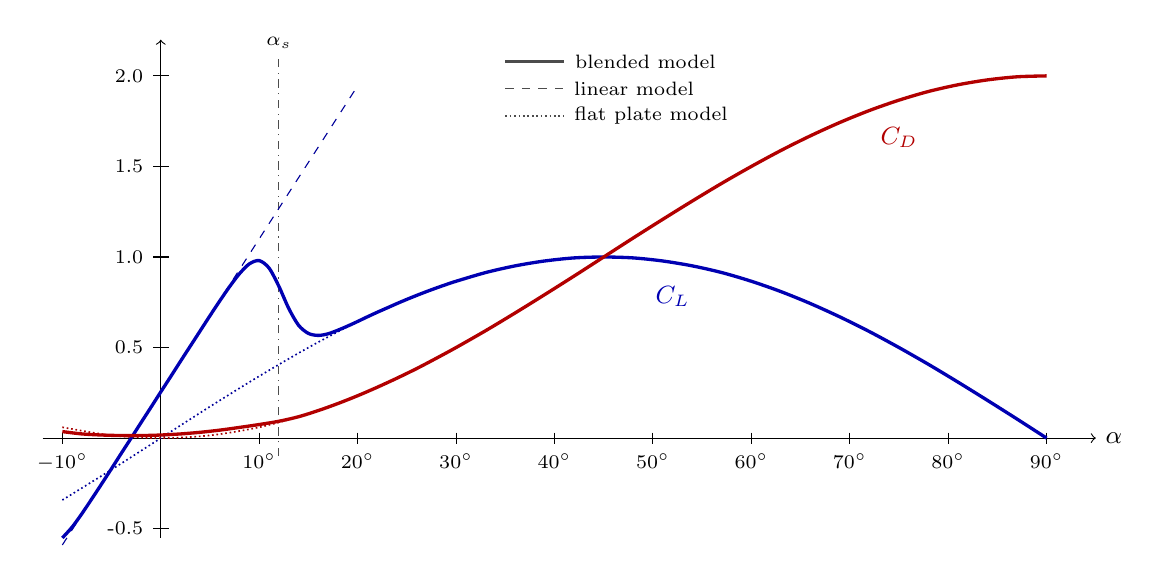
\begin{tikzpicture}[x=0.125cm, y=2.3cm, thick, every node/.style={font=\small}]
% axes
\draw[->, thin] (-12,0) -- (95,0) node[right]{$\alpha$};
\draw[->, thin] (0,-0.55) -- (0,2.2);
\foreach \a in {-10,10,20,30,40,50,60,70,80,90} {
    \draw[thin] (\a,0.03) -- (\a,-0.03) node[below, font=\scriptsize]{$\a^{\circ}$};
}
\foreach \v in {-0.5,0.5,1.0,1.5,2.0} {
    \draw[thin] (0.8,\v) -- (-0.8,\v) node[left, font=\scriptsize]{\v};
}
% stall angle
\draw[thin, dash dot, gray!60!black] (12.0,-0.1) -- (12.0,2.1) node[above, font=\scriptsize, text=black]{$\alpha_s$};
% linear and flat plate models
\draw[thin, dashed, blue!60!black] (-10,-0.590) -- (20,1.945);
\draw[semithick, densely dotted, blue!60!black] plot[smooth] coordinates {(-10,-0.342) (-5,-0.174) (0,0.000) (5,0.174) (10,0.342) (15,0.500) (20,0.643) (25,0.766) (30,0.866) (35,0.940) (40,0.985) (45,1.000)};
\draw[semithick, densely dotted, red!65!black] plot[smooth] coordinates {(-10,0.060) (-5,0.015) (0,0.000) (5,0.015) (10,0.060) (15,0.134) (20,0.234) (25,0.357) (30,0.500)};
% CL
\draw[very thick, blue!70!black] plot[smooth] coordinates {(-10,-0.551) (-9,-0.491) (-8,-0.416) (-7,-0.335) (-6,-0.252) (-5,-0.168) (-4,-0.083) (-3,0.001) (-2,0.086) (-1,0.170) (0,0.255) (1,0.339) (2,0.424) (3,0.508) (4,0.592) (5,0.676) (6,0.758) (7,0.837) (8,0.908) (9,0.962) (10,0.980) (11,0.939) (12,0.838) (13,0.716) (14,0.623) (15,0.578) (16,0.567) (17,0.576) (18,0.596) (19,0.619) (20,0.644) (21,0.670) (22,0.695) (23,0.719) (24,0.743) (25,0.766) (26,0.788) (27,0.809) (28,0.829) (29,0.848) (30,0.866) (33,0.914) (36,0.951) (39,0.978) (42,0.995) (45,1.000) (48,0.995) (51,0.978) (54,0.951) (57,0.914) (60,0.866) (63,0.809) (66,0.743) (69,0.669) (72,0.588) (75,0.500) (78,0.407) (81,0.309) (84,0.208) (87,0.105) (90,0.000)};
% CD
\draw[very thick, red!70!black] plot[smooth] coordinates {(-10,0.036) (-8,0.023) (-6,0.017) (-4,0.014) (-2,0.014) (0,0.017) (2,0.023) (4,0.032) (6,0.044) (8,0.059) (10,0.075) (12,0.093) (14,0.118) (16,0.152) (18,0.191) (20,0.234) (22,0.281) (24,0.331) (26,0.384) (28,0.441) (30,0.500) (33,0.593) (36,0.691) (39,0.792) (42,0.895) (45,1.000) (48,1.105) (51,1.208) (54,1.309) (57,1.407) (60,1.500) (63,1.588) (66,1.669) (69,1.743) (72,1.809) (75,1.866) (78,1.914) (81,1.951) (84,1.978) (87,1.995) (90,2.000)};
\node[blue!70!black, font=\small] at (52,0.78) {$C_L$};
\node[red!70!black, font=\small] at (75,1.66) {$C_D$};
% legend
\draw[very thick, black!70] (35,2.08) -- (41,2.08) node[right, font=\scriptsize, text=black]{blended model};
\draw[thin, dashed, black!70] (35,1.93) -- (41,1.93) node[right, font=\scriptsize, text=black]{linear model};
\draw[semithick, densely dotted, black!70] (35,1.78) -- (41,1.78) node[right, font=\scriptsize, text=black]{flat plate model};
\end{tikzpicture}
\caption[Lift and drag coefficients of the aerodynamic model]{Lift and drag coefficients of the aerodynamic model for the wing of the reference drone (NACA 3416 section, aspect ratio 7.5). The dashed line is the linear model \eqref{eq:aero-linear} (shown for the lift only), the dotted lines are the flat plate model \eqref{eq:aero-plate}, and the solid lines are their blend \eqref{eq:aero-blend} around the stall angle $\alpha_s = 12.0^{\circ}$ of the finite wing. The maximum lift coefficient is 0.98 and the best lift to drag ratio of the isolated wing is 18.7.}
\label{fig:aero-coefficients}
\end{figure}

The parameters of the section, $\alpha_0$, $\alpha_s^{\mathrm{2D}}$, $C_{D_0}$ and $\mathit{Re}_{\mathrm{nom}}$, follow from the airfoil. The table from which they are read (\autoref{subsec:genesis-aero}) was computed from polars obtained with XFOIL \cite{drela1989xfoil} over a sweep of Reynolds numbers. The slope of the section is fixed at $C_{\ell_\alpha} = 0.11$ per degree, the value that thin airfoil theory predicts to within one percent. The fuselage produces no lift and a constant drag coefficient of 0.35 referred to its own reference area.

\paragraph{Forces and points of application.} With the dynamic pressure $\tfrac{1}{2}\rho V^2$, the air density $\rho = 1.225$~kg/m$^3$ and the area $S$ of the element, lift and drag are
\begin{equation}
L = \tfrac{1}{2}\,\rho V^2 S\, C_L \cos^2\!\beta, \qquad D = \tfrac{1}{2}\,\rho V^2 S\, C_D \cos^2\!\beta,
\label{eq:aero-lift-drag}
\end{equation}
where the factor $\cos^2\beta$, applied to the wing and to the elevator, expresses the classical result that only the component of the flow normal to the span of a surface loads it. The two magnitudes are assembled in wind axes and rotated into the frame of the surface through the two aerodynamic angles,
\begin{equation}
\vect{F} = \mat{R}_z(\beta)\, \mat{R}_y(\alpha)\, \bigl( D,\; 0,\; L \bigr)^{\top},
\label{eq:aero-force}
\end{equation}
with $\mat{R}_y$ and $\mat{R}_z$ the elementary rotations about the $y$ and $z$ axes of the frame. The rudder is treated as a wing turned by ninety degrees: its incidence is the sideslip angle, its coefficients are evaluated at $\beta$, and its lift acts as a side force along $y$. The force is applied at the \emph{centre of pressure} of the surface, which for an attached flow lies at the quarter of the chord and moves towards the middle of the chord as the flow separates:
\begin{equation}
\frac{x_{\mathrm{cp}}}{\bar c} = \frac{1}{4} + \frac{1}{4}\, \frac{\lvert\alpha\rvert}{\pi/2} .
\label{eq:aero-cp}
\end{equation}
Since the rigid body solver receives a force and a point, the aerodynamic moments of the drone are never modelled as such: the pitching moment that trims the aircraft, the rolling moment of a differential twist and the yawing moment of an asymmetric sweep all arise as moments of the forces \eqref{eq:aero-force} about the centre of mass, and they change with the body because the points of application do.

\paragraph{Interaction between the elements.} Two interactions are modelled, both directed at the tail. The first is the \emph{downwash} of the wing: a wing that produces lift deflects the flow behind it downwards, and the elevator works in that deflected flow. Its angle of attack is reduced by the downwash angle that lifting-line theory predicts at the wing,
\begin{equation}
\alpha_{\mathrm{t}} = \alpha - \varepsilon, \qquad \varepsilon = k_{\varepsilon}\, \frac{C_{L,\mathrm{w}}}{\pi\, \mathit{AR}_{\mathrm{w}}},
\label{eq:aero-downwash}
\end{equation}
where $C_{L,\mathrm{w}}$ is the lift coefficient that the wing half on the same side has at that same substep, $\mathit{AR}_{\mathrm{w}}$ the aspect ratio of the wing and $k_{\varepsilon} = 1$. This couples the two surfaces the way it does on a real aircraft (an increase of wing lift reduces the effectiveness of the tail) and makes the two halves of the elevator work differently when the two halves of the wing do. For this reason the kernel evaluates the elements in a fixed order: the propeller first, then the wing and the fuselage, then the tail. The second interaction is the \emph{slipstream} of the propeller, whose induced velocity, given below, corrects the axial component of the flow seen by the elevator through a gain $k_s$.

\paragraph{Propeller.} The throttle command $u \in [0,1]$ passes through a first order lag that represents the inertia of the motor and of the propeller,
\begin{equation}
\tilde u_{k+1} = \tilde u_k + \frac{\Delta t}{\Delta t + 1/(2\pi f_c)}\,\left(u_k - \tilde u_k\right),
\label{eq:prop-lag}
\end{equation}
with a cut-off frequency $f_c = 0.32$~Hz, and the filtered command sets the rotation speed $n = \tilde u\, n_{\max}$ (in revolutions per second), where $n_{\max}$ is the smaller of the no-load speed of the motor, $K_V U / 60$ for a speed constant $K_V = 2300$~rpm/V and a supply voltage $U = 7.4$~V, and of the speed at which the propeller delivers its maximum static thrust $T_{\max} = 5.2$~N. The thrust of a propeller of diameter $d$ falls as the aircraft flies faster, because the blades meet the air at a lower incidence; this is described by a thrust coefficient that decreases with the \emph{advance ratio} $J$ \cite{mccormick1995aerodynamics}:
\begin{equation}
J = \frac{V_a}{n\, d}, \qquad T = \rho\, n^2 d^4\, C_{T_0} \max\!\left(0,\; 1 - c_1 J - c_2 J^2\right),
\label{eq:prop-thrust}
\end{equation}
with $V_a$ the component of the relative wind along the axis of the propeller, $C_{T_0} = 0.093$, $c_1 = 0$ and $c_2 = 2.148$, and $T$ limited to the interval $[0, T_{\max}]$. The thrust acts along the axis, together with a reaction torque $\kappa T$ about it, $\kappa = 0.01$~m. The velocity induced in the slipstream follows from the momentum theory of the actuator disc of area $A = \pi d^2/4$:
\begin{equation}
v_{\mathrm{ind}} = \frac{1}{2}\left( -V_a + \sqrt{V_a^2 + \frac{2T}{\rho A}} \right).
\label{eq:prop-induced}
\end{equation}

\paragraph{Coupling and safeguards.} At each substep the forces of all elements, with their points of application, are transformed to the world frame and accumulated on the links of the rigid body as forces and moments. Three safeguards protect the explicit coupling. The speed $V$ that enters the coefficients is limited to 40~m/s, the force on each element is limited to 30~N, several times the weight of the drone, and values that are not finite are replaced by zero before they reach the rigid body solver. In a parallel simulation this last point is not cosmetic: the environments of a scene are advanced by the same kernels on shared arrays, and a single environment whose state diverges can otherwise spread its invalid values to the rest of the batch.

\paragraph{Limits of the model.} The simplifications named in \autoref{subsec:genesis-aero} are stated here in full. The model is quasi-steady: forces depend on the instantaneous flow only, so unsteady effects such as dynamic stall or the lag of the downwash in reaching the tail are absent. Each surface carries a single lumped force, so the distribution of the load along the span, and with it the progressive stall of a twisted or swept wing, is not resolved. The relative wind \eqref{eq:aero-angles} of every element is computed from the velocity of the centre of mass: the additional flow that a rotation of the body induces at a surface far from the centre of mass is neglected, and the rotations of the drone are damped only indirectly, through the change of incidence they produce. Interference is limited to the two effects described above. Finally, the air is at rest: there is no wind and no turbulence other than the noise described in \autoref{app:aero-noise}.

\section{Aerodynamic Noise}
\label{app:aero-noise}

The aerodynamic noise of \autoref{subsec:genesis-noise} perturbs the force \eqref{eq:aero-force} of every lifting surface in magnitude and in direction before it is applied:
\begin{equation}
\begin{gathered}
\tilde{\vect{F}} = \lVert \vect{F} \rVert \left(1 + \sigma_m\, s\, \xi\right) \frac{\hat{\vect{F}} + \sigma_d\, s\, \vect{g}_{\perp}}{\lVert \hat{\vect{F}} + \sigma_d\, s\, \vect{g}_{\perp} \rVert}, \\
s(\alpha, \beta) = 1 + 3 \left( \frac{\min\!\left(\sqrt{\alpha^2 + \beta^2},\, \pi\right)}{\pi} \right)^{\!2},
\end{gathered}
\label{eq:aero-noise}
\end{equation}
where $\hat{\vect{F}}$ is the unit vector of $\vect{F}$, $\xi$ a standard normal variable, $\vect{g}_{\perp}$ a random unit vector orthogonal to $\vect{F}$, and $\sigma_m = \sigma_d = 0.05$. The scale $s$ grows from 1 in aligned flow to 4 in fully reversed flow. The centre of pressure is displaced at the same time by a random offset whose standard deviation is a fraction $\sigma_{\mathrm{cp}}\, s / 4$ of the chord, with $\sigma_{\mathrm{cp}} = 0.01$, limited to 15\% of the chord.

\section{Collision Test and Forest Statistics}
\label{app:forest-math}

\paragraph{Collision.} Let $(x_b, y_b)$ be the position of the centre of a trunk in the horizontal frame centred on the drone and aligned with its heading, $b$ the combined span of the two wing panels and $\phi$ the roll angle of the drone. The drone has hit the trunk when
\begin{equation}
\lvert x_b \rvert \le r + \tau \qquad \text{and} \qquad \lvert y_b \rvert \le \frac{b}{2}\cos\phi + r + \tau ,
\label{eq:forest-collision}
\end{equation}
where $\tau$ is the safety margin of \autoref{sec:flight-environment}.

\paragraph{Survival of a blind flight.} Consider a drone that flies straight and blind. It touches a trunk whenever a centre falls in the strip of width $w = b + 2r$ swept by its wing, and since the positions are independent, the probability that it is still flying at $x$ is
\begin{equation}
S(x) = \exp\!\left( -\frac{w}{W} \int_0^x \lambda(\xi)\, d\xi \right),
\label{eq:forest-survival}
\end{equation}
which for a constant $\lambda$ is an exponential law: the distance covered has a standard deviation equal to its mean.

With the profile \eqref{eq:forest-density} the survival \eqref{eq:forest-survival} of the blind straight flight becomes
\begin{equation}
S(x) = \exp\!\left[ -\frac{w}{W} \left( \lambda_0\, x + \frac{\lambda_1 - \lambda_0}{2L}\, x^2 \right) \right],
\label{eq:forest-survival-growing}
\end{equation}
whose quadratic term makes the risk grow with the distance already flown.

\paragraph{Sampling of a growing forest.} The coordinate of a tree along the course is drawn from the density proportional to \eqref{eq:forest-density} by inverting its cumulative distribution, which for a linear profile has a closed form: if $u$ is uniform in $[0,1]$,
\begin{equation}
x = L\; \frac{\sqrt{\lambda_0^2 + u\left(\lambda_1^2 - \lambda_0^2\right)} - \lambda_0}{\lambda_1 - \lambda_0} .
\label{eq:forest-inverse-cdf}
\end{equation} Since the forests of a batch share one tensor and may have different numbers of trees, the shorter lists are padded with inactive trees parked outside the corridor, where they can be neither seen nor hit.

\section{Uniform and Latin Hypercube Forests}
\label{app:forest-generators}

Two forest generators were written besides the growing density generator of \autoref{subsec:forest-growing}. They share its corridor and its trees and differ only in the law of the positions. The first was used for internal tests, and the second was explored and then abandoned. The figures show both in the same corridor and with nearly the same number of trees as \autoref{fig:forest-growing}, so that the three forests can be compared directly.

\subsection{Uniform Density Forests}
\label{subsec:forest-uniform}

The simplest forest places a fixed number $N$ of trees independently and uniformly in the rectangle $[0, L] \times [-W/2, W/2]$ (\autoref{fig:forest-uniform}). The density is the same everywhere: $N/(LW)$ trees per square metre or, in the unit used throughout this thesis, $\lambda = N/L$ trees per metre of course.

\begin{figure}[htbp]
\centering
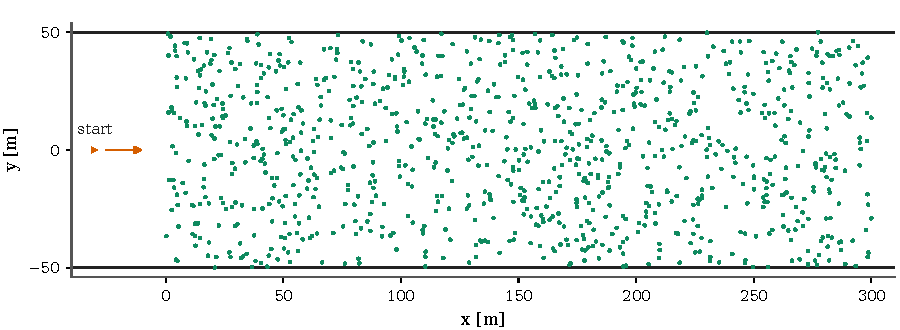
\includegraphics[width=\textwidth]{images/04_Simulation_Environment/forest_uniform.pdf}
\caption[A uniform density forest]{A uniform density forest seen from above: 975 trees placed independently and uniformly in a corridor of 300~m by 100~m. Trunks are drawn to scale. The thickets and the clearings are what independent positions look like.}
\label{fig:forest-uniform}
\end{figure}

A uniform forest is statistically the same at every point of the course, and this is what makes it useful for testing. It was used to verify the depth sensor and the collision test, to debug the flight of new bodies, and to observe how a controller behaves at one given density, without the confounding effect of a forest that changes as the drone advances.

The same property makes it a poor instrument for measuring. The difficulty of a uniform forest is a single number that has to be chosen in advance, and no choice suits a population of bodies of very different ability. In a sparse forest every competent body reaches the end and the progress saturates. In a dense forest every body fails within a few metres. Between these extremes the measure is dominated by chance. The cleanest way to see this is to consider a drone that flies straight and blind. Since the positions of the trees are independent, the risk of hitting one in the next metre is the same whatever the distance already flown. The distance covered before the collision therefore follows the exponential law of \eqref{eq:forest-survival}, whose standard deviation equals its mean. In the forest of \autoref{fig:forest-uniform}, with $b = 1.4$~m for the reference drone, that mean is 11~m, measured from the first tree. A controller that sees the trees does much better than this, but it inherits the structure of the problem. In a stationary forest the length of a flight has a large memoryless component, and many flights are needed before two bodies can be told apart.

\subsection{Latin Hypercube Forests}
\label{subsec:forest-latin}

Independent positions have a cost. Nothing prevents two trunks from being drawn on top of each other, or a few of them from lining up so closely that they form a wall. The effect is not marginal. For independent positions of areal density $n$, the probability that a tree has a neighbour closer than a distance $d$ is $1 - e^{-n\pi d^2}$. At one tree every 25~m$^2$, a density that the forests of this work reach in their last part, a quarter of the trunks overlap another trunk ($d = 2r$). Almost two thirds of them are separated from their nearest neighbour by a gap narrower than the width $b$ of the reference drone ($d = 2r + b$). Chains of such pairs form barriers several metres wide (\autoref{fig:forest-overlaps}, left). A flight that ends against one of them says little about the body or about the controller. This luck of the draw is one of the sources of the noise that every comparison in this thesis has to average out.

\begin{figure}[htbp]
\centering
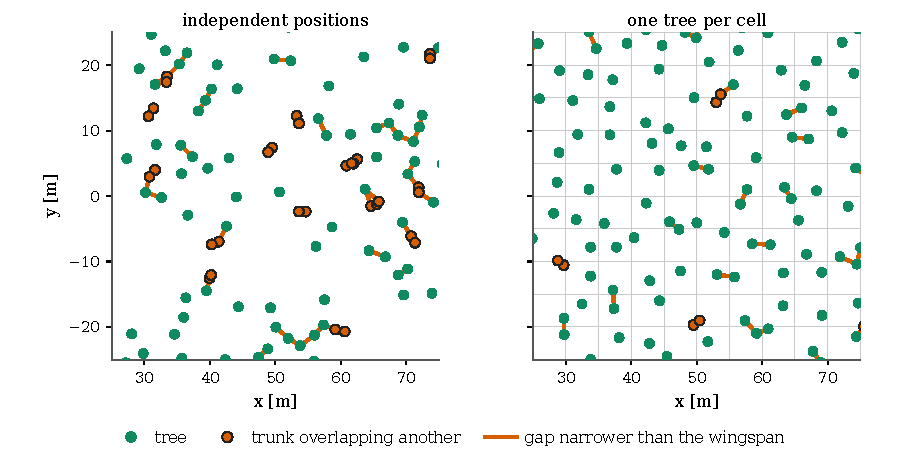
\includegraphics[width=\textwidth]{images/04_Simulation_Environment/forest_random_vs_stratified.pdf}
\caption[Independent and stratified positions at the same density]{Independent and stratified positions at the same density, one tree every 25~m$^2$, in a window of 50~m by 50~m with trunks to scale. With independent positions 25\% of the trunks overlap another and 64\% leave a gap narrower than the width $b = 1.4$~m of the reference drone; with one tree per cell the two figures fall to 6\% and 39\% (averages over 200 forests).}
\label{fig:forest-overlaps}
\end{figure}

The stratified generator was written to remove this effect. It borrows the idea of \emph{Latin hypercube sampling} \cite{mckay1979comparison}, the classical device for spreading random samples evenly over a domain: the domain is divided into strata, and the samples are forced to occupy the strata evenly while remaining random inside them. Here the corridor is tiled with rectangular cells, and exactly one tree is placed in each cell, at a position uniform within it. To keep the density growing along the course, the cells shrink. The course is cut into columns whose width decreases linearly from $s_0$ at the entrance to $s_1$ at the end, rescaled so that they tile the length $L$ exactly. Each column is then cut into equal rows whose height follows the same interpolation (\autoref{fig:forest-latin}). The name is used loosely. In a Latin hypercube proper each row and each column of the grid holds exactly one sample. Here every cell does, which is the stronger form of stratification also known as jittered sampling.

\begin{figure}[htbp]
\centering
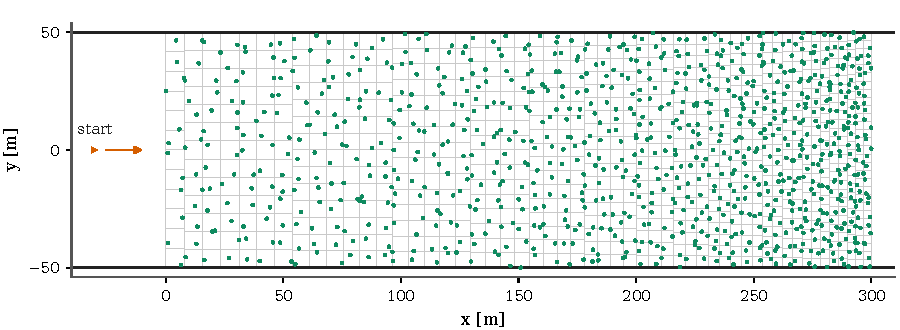
\includegraphics[width=\textwidth]{images/04_Simulation_Environment/forest_latin.pdf}
\caption[A Latin hypercube forest]{A Latin hypercube forest seen from above, with its cells. The cells shrink from 8~m to 3.4~m along the course and each holds exactly one tree, for 988 trees in total, about as many as in \autoref{fig:forest-uniform} and \autoref{fig:forest-growing}.}
\label{fig:forest-latin}
\end{figure}

The stratification does what it was meant to do. At the same density the overlapping trunks fall from 25\% to 6\%, and the gaps narrower than the width $b$ from 64\% to 39\% (\autoref{fig:forest-overlaps}, right). No region can be crowded, because at most four trees can meet around the corner shared by four cells. No region can be empty, because every cell is occupied. The number of trees is also identical in all the forests of a batch.

It was nevertheless abandoned, because what it removes is part of the task. A forest drawn in this way is tidy: the trees are almost evenly spaced and every gap is about one cell wide. The thickets and the clearings that a real forest has, and that \autoref{fig:forest-uniform} and \autoref{fig:forest-growing} show, are gone. A body and a controller selected in such a forest are selected in the presence of a regularity that no real environment offers, and a search could come to rely on it. The results of this thesis are therefore obtained in growing density forests with independent positions (\autoref{subsec:forest-growing}).

\section{Mass Model and Propeller Power of the Drone}
\label{app:drone-mass-power}

\paragraph{Masses.} The fuselage is a foam shell 15~mm thick, and the wing and tail surfaces are solid foam panels whose thickness follows their airfoil section, all with a density of 20~kg/m$^3$ (reduced by a fill factor of 0.68 for the surfaces). The fixed masses are 200~g for the battery and the electronics, 30~g for the camera, 41.5~g for the motor and the propeller, 90~g for the six servomotors and 40~g for hinges and fittings.

\paragraph{Propeller power.} The power absorbed by the propeller follows from its rotation speed $n$ and its advance ratio $J$, with the same kind of law as the thrust \eqref{eq:prop-thrust}:
\begin{equation}
P_{\mathrm{prop}} = \rho\, n^3 d^5\, C_{P_0} \max\!\left(0,\; 1 - c'_1 J - c'_2 J^2\right),
\label{eq:drone-prop-power}
\end{equation}
with $C_{P_0} = 0.044$, $c'_1 = 0$ and $c'_2 = 1.104$.
